\section{Dynamische Geschäftsprozesse auf Basis von Ereignisverarbeitung}\label{sec:Kombi}
Bei der Automatisierung von Geschäftsprozessen und deren dynamischen Eigenschaften wächst, der Bedarf auf kritische Ereignisse in Echtzeit und ohne Latenzen zu reagieren.
Um den steigenden Anforderungen nach Echtzeitmanagement von Geschäftsprozessen unter Betrachtung relevanter Ereignisse zur Laufzeit gerecht zu werden, stellt die Integration von Ereignisverarbeitungskonzepten in die serviceorientierte Geschäftsprozessautomatisierung ein geeignetes Mittel dar. Die Vorteile für ein Unternehmen bei einer solchen Vervollständigung von Geschäftsprozessautomatisierung mit Konzepten der Ereignisverarbeitung sind im Wesentlichen durch folgenden Charakteristika fundiert:

\subsection{Merkmale und Kriterien}

\begin{figure}[H]
	\centering 
    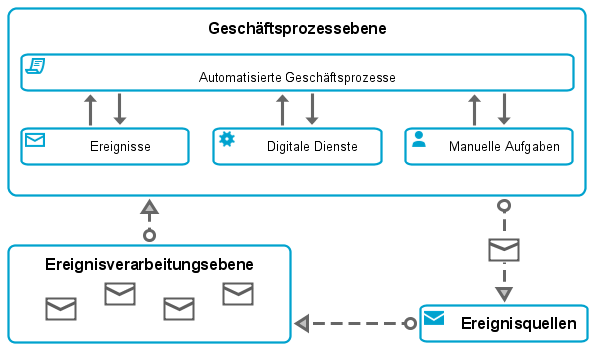
\includegraphics[width=\textwidth]{img/dynamicbp.png}	
    \caption[Ebenen dynamischer Geschäftsprozesse]
    {Ebenen dynamischer Geschäftsprozesse \protect\footnotemark}
    \label{fig:Ebenen dynamischer Geschäftsprozesse}
\end{figure}
\footnotetext{in Anlehnung an \citeauthor{Vidackovic.2014} \citeyear{Vidackovic.2014} \cite{Vidackovic.2014} }


\missingfigure{Tabelle Kriterien für das Management dynamischer Geschäftsprozesse}

\subsection{Gegenüberstellung vorhandener Forschungsansätze}

\todo{Etwas einfallen lassen}
\cite{Wolf.2016}
\cite{RobraBissantz.2009}
\cite{Bruns.2010}S.37